\documentclass{lab_sheet}
\usepackage[inline]{enumitem}
\begin{document}
\titlePage{Study of Network Architecture with Network Devices and Cables}{October 8, 2020}
\pagenumbering{gobble}
\tableofcontents
\pagebreak
\listoftables
\pagebreak
\listoffigures
\pagebreak
\pagenumbering{arabic}
\section{Objectives}
\begin{itemize}
    \item Familiarization with various layers of layered network architecture and need of logical addressing
    \item Familiarization with various network devices viz. Hub, Bridge, Router, Switch, Repeater, etc.
    \item Familiarization with crimping tool, RJ-45 connector, path panel, and various color-coding schemes of an UTP network cable.
    \item Familiarization with preparation, testing and operation of straight through and crossover cables along with their uses.
\end{itemize}
\section{Required Tools}
\subsection{Crimping tool}
Literal meaning of a crimp is an action of compressing something to form small folds or ridges. A crimping tool is essentially used to join two metallic pieces by deforming any one or in some cases both to fix them together. It is generally used to mount a connector on the end of a cable by crimping the exterior coating of a cable and creating an electrical connection between the metallic pieces of a connector and the cable. It also comes with a handy cutting section to cut and strip the exterior protective jacket of a cable.
\begin{figure}[H]
    \centering
    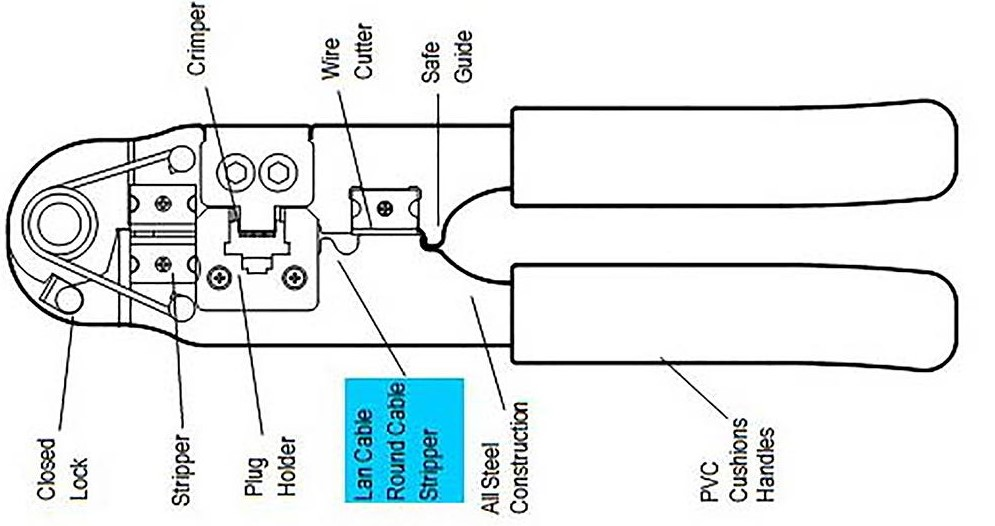
\includegraphics[scale=0.3]{Figures/climper.jpg}
    \caption{Crimping tool}
    \label{fig:crimpingtool}
\end{figure}
\subsection{Network devices}
Various network devices such as hub, switch, bridge, repeater, router, etc. are essential parts of a network architecture.
\subsection{Rj-45 connectors and patch panel}
Rj-45 is a standardized connector used mostly for ethernet networks. It contains eight pins such that an UTP cable is crimped onto these pins to establish a connection. Not all pins are essential for communication in current standards since only two pairs are used for the transmitting and receiving purpose.\\
A patch panel is basically an array of ports on a single panel mostly used for bundling multiple ports to connect incoming and outgoing cables more effectively. It can be as small as a single port patch panel or large with hundreds of ports depending on the requirement.
\begin{figure}[H]
    \centering
    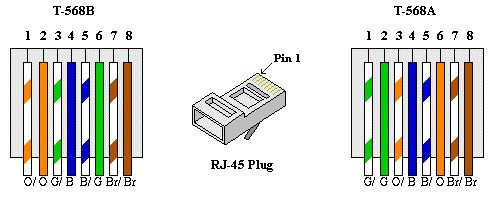
\includegraphics[scale=0.7]{Figures/rj45.jpg}
    \caption{Registered Jack 45 with Class A and Class B color-schemes}
    \label{fig:rj45}
\end{figure}
\subsection{Pieces of UTP cable (CAT 5 or CAT 6)}
An UTP cable is one of the most used types of cables for LAN setups due to its cheap price and reasonable speed. A CAT 5 cable is pretty much overlooked in comparison to CAT 5 enhanced or a CAT 6 cable due to significant improvements in transfer speed and reduction of crosstalk. Both categories of UTP cables are used with a RJ-45 cable that enables the interchanging of both the setups.
\subsection{LAN cable tester}
LAN cables are generally an UTP cable fitted with RJ-45 connectors on both ends. The connection of the required wires in either the T568A or T568B color code standards has to be confirmed for proper cable testing. A network is incomplete without a proper electrical connection between the two ends of the LAN cable. For a wire of short length, a multimeter can be used to check for connections of individual pins but this can be a real hassle if the two ends of the cable are farther apart. For this, a LAN cable tester is used. A LAN cable tester comes in a pair and each one has a port for plugging in one end of LAN cable to be tested. LEDs are fitted on both the testing handhelds such that they blink serially on an active connection. The serial blinking of LEDs is noted on both the ends and later confirmed to make testing conclusion.
\begin{figure}[H]
    \centering
    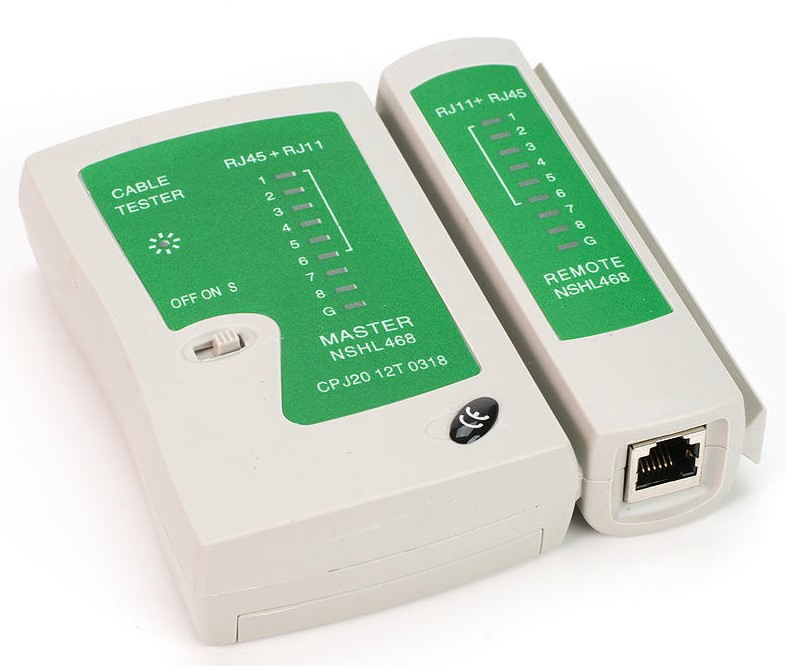
\includegraphics[scale=0.3]{Figures/tester.jpg}
    \caption{Battery powered LAN cable tester}
    \label{fig:tester}
\end{figure}
\section{Procedure}
Since the lab experiments were carried out virtually, the required tools were demonstrated by the lecturer. The activities were carried out virtually but with enough description and detail such that we were able to understand the procedures involved.
\subsection{Testing a LAN cable using LAN cable tester}
A LAN cable tester was used to test for electrical connectivity between the two ends of the wire.
\begin{enumerate}
    \item Firstly, the cable tester was turned on. One end of the LAN cable was inserted into the port of the transmitting handheld. It's generally denoted as TX.
    \item The other end of the cable was inserted into the RX of the receiving handheld.
    \item The tester had 8 LEDs equivalent to the 8 pins on the cable. The tester sends a signal from the transmitting end to the other serially from pin 1 and tests for the receiving signal to test the connection. The blinking of LEDs on both the ends were noted and then compared to know the connection status.
\end{enumerate}
\subsection{Crimping an RJ-45 connector on an UTP cable}
\begin{enumerate}
    \item Firstly, the connector on the faulty LAN cable was cut off. The exterior jacket of the cable was then stripped using the stripping section of the crimping tool. About 25 mm of the jacket was stripped by first fixing the cable in the stripping section, then the tool was squeezed tightly. Once a firm grip was established, the tool was rotated around in approximate semi-circles to cut off a clean section. The jacket was removed leaving behind exposed twisted pairs of wires.
    \item The wires were untwisted and straightened. Since there was a separator core, it was cut out using the crimping tool. The wires were then arranged in order according to the need of a straight-through or crossover cable configuration.
    \item Once the wires were placed in order, they were cut off using the cutting section of the crimping tool. This was done to get an equal length of wires leaving behind about 0.5 inch of wires outside the jacket.
    \item The wires were then inserted into the RJ-45 connector such that the jacket itself went inside the connector body for proper protection. Before crimping, the insertion was verified such that each wire was pushed in their own space within the connector.
    \item Finally, the connector body was inserted into the crimping section of the crimping tool and it was squeezed to crimp the wires onto the connector.
\end{enumerate}
\section{Observation}
LAN tester showed that there was a fault in connection on the cable that the lecturer used. The LEDs 1 and 2 on the handhelds lit up in switched order indicating that the pin 1 and pin 2 of the two terminals of the LAN cable had been incorrectly crimped, which was true since the cable was pre-determined to be faulty. This led us to cut off the connector and re-crimp it. Once re-crimped, the LAN tester showed no signs of fault.
\section{Exercises}
\problem{What is layered network architecture? Why layering is important?}
A layered network architecture is a set of rules defined such that they govern the interaction and inter-connection of various devices on the network along with the protocols, standards and data exchange formats used. Layered architecture in a more general sense is one where the data moves from one predefined level of processing to a different level such that each layer separates the functionality into separate levels for effective communication between two nodes. It is a separation of network into functional layers that communicate with one another in a hierarchical format such that a  layer is capable of interacting with only the layers above and below itself.\\
The importance of layering in a network are listed as:
\begin{enumerate}
    \item Layering allows abstraction in network. Say, a message from the application layer is sent to the transport layer where source port and destination port numbers are added to the packet. This is then transferred to the network layer which adds the IP addresses into the packet. Here the individual layers don't intervene on other layers hence creating abstraction.
    \item Debugging is easier in a layered network architecture. Say an error occurs while looking for the IP address of an end point. The error can be easily sorted since the point of occurrence is known.
    \item Layering helps in standardized networking protocols to be used. This way multiple hardware manufacturers and software developers have a common working ground such that they can develop network devices and software that can be communicate over the network.
\end{enumerate}
\problem{What is protocol? List out ten different standard protocols having at least one in each layer of TCP/IP
reference model.}
A protocol is a predefined set of instructions that detail how data should be transmitted between two devices on a network. It can be thought of as an agreement that the devices and layers in a network make such that it defines how data should be structured, transmitted and received. Protocols are established abiding by the industry standard by networking or IT organizations such as IEEE, ISO, ITU, W3C, IETF.  Without protocols devices wouldn't have a fixed guideline to communicate hence disrupting the idea of an effective and versatile network.\\
The list of ten standard protocols with each layer of TCP/IP reference model having at least one are:
\begin{table}[H]
    \centering
    \begin{tabular}{|C{4cm}|C{7.5cm}|}
        \hline
        \textbf{TCP/IP Layer} & \textbf{Protocols}         \\ \hline
        Application           & \begin{itemize}
            \item Domain Network System (DNS)
            \item File Transfer Protocol (FTP)
        \end{itemize}  \\ \hline
        Transport             & \begin{itemize}
            \item Transmission Control Protocol (TCP)
            \item User Datagram Protocol (UDP)
        \end{itemize}  \\ \hline
        Internet              & \begin{itemize}
            \item Internet Protocol (IP)
            \item Internet Control Message Protocol (ICMP)
        \end{itemize} \\ \hline
        Data Link             & \begin{itemize}
            \item IEEE 802.2
        \end{itemize} \\ \hline
        Physical              & \begin{itemize*}
            \item IEEE 802.3
            \item RS-232
            \item IEEE 802.5
        \end{itemize*} \\ \hline
    \end{tabular}
    \caption{Standard protocols with each layer of TCP/IP reference model having at least one protocol}
\end{table}
\problem{List out the devices that can work up to physical, data link, network and application layer.}
The devices that can work in each of physical, data link, network and application layer are:
\begin{table}[H]
    \centering
    \begin{tabular}{|C{4cm}|C{7.5cm}|}
        \hline
        \textbf{Working Layer} & \textbf{Devices}           \\ \hline
        Physical               & \begin{itemize}
            \item Repeaters
            \item Hubs
            \item Cables
        \end{itemize} \\ \hline
        Data Link              & \begin{itemize}
            \item Modem
            \item Network Interface Card (NIC)
            \item Bridges
            \item Layer 2 Switch
        \end{itemize} \\ \hline
        Network                & \begin{itemize}
            \item Brouters (Bridge Router)
            \item Routers
            \item Layer 3 Switch
        \end{itemize} \\ \hline
        Application            & \begin{itemize}
            \item Personal computer
            \item Servers
            \item Mobile phones
            \item Gateways
        \end{itemize} \\ \hline
    \end{tabular}
    \caption{Devices that can work up to physical, data link, network and application layer}
\end{table}
A switch works on both the data link and network layer depending on its construction. Thus, there are switches known as Layer 2 switch and Layer 3 switch. A layer 2 switch sends frames to the destination depending on the MAC address whereas the layer 3 switch uses the IP address. A layer 3 switch is most widely used in VLAN setups and can communicate outside the network in addition to internal communication unlike the layer 2 switch which only communicates within the network.
\problem{Compare the devices (showing the similarities as well as differences):}
The similarities and differences between the noted network devices are presented in separate tables.
\subproblem{Repeater and Hub}
\difference{Repeater}{Hub}{Similarities}{Working layer of OSI model& Physical layer                                                           & Physical layer                                                                                                      \\ \hline
    Functionality & Used to repeat a fading signal such that it extends the LAN range.       & Can be used to repeat a fading signal.                                                                              \\ \hline
    Routing  & Has only one output port so can't direct signal to specific destination. & Has multiple output ports but can't select a specific destination rather sends the signal to all connected devices.
    \\ \hline
}
\difference{Repeater}{Hub}{Differences}{Number of ports & 2 ports (1 incoming and 1 outgoing)                                & Multiple ports (Generally 4, 8, 16 or 32) \\
    \hline
    Usage           & Only used to regenerate fading signals to extend the LAN distance. & Used to connect multiple wires from various nodes such that all connect hosts have the same collision domain. \\ \hline}
\subproblem{Bridge and Switch}
\difference{Bridge}{Switch}{Similarities}{
    Working layer of OSI model          & Data link layer                                      & Data link layer                                       \\ \hline
    Usage                      & Used to connect different LAN segments.              & Used to connect different LAN segments.               \\ \hline
    Filtering                  & Can filter data and select the required destination. & Used essentially for their filtering capabilities. \\ \hline
    Packet filtered based on& MAC address                                          & MAC address                                           \\ \hline}
\difference{Bridge}{Switch}{Differences}{Number of ports        & Has either 2 or 4 ports.        & Can have multiple ports.                                        \\ \hline
    Switching method       & Can use only store and forward. & Uses either of store and forward, cut-through or fragment-free. \\ \hline
    Error                  & Can't perform error checking.   & Perform error checking.                                         \\ \hline
    Packet forwarding & Software based                & Hardware based (Eg. ASICS)
    \\
    \hline
    Availability of buffer & No                              & Yes (for each link)                                             \\ \hline}
\subproblem{Repeater and Bridge}
\difference{Repeater}{Bridge}{Similarities}{Connection of LANs & Connects two portions of LAN such that the signal is regenerated and LAN distance is increased. & Connects two segments of LAN hence the name 'bridge'. \\ \hline}
\difference{Repeater}{Bridge}{Differences}{ Working layer of OSI model & Physical layer                                                                                   & Data link layer                                                 \\ \hline
    Destination                & Can't locate the destination rather just forwards the signal to any device on the outgoing port. & Uses MAC address to locate the destination to forward a frame.  \\ \hline
    Collision domain           & If collision occurs, it is forwarded to the other segment causing the same issue.                & Bridge doesn't forward a collision from one segment to another. \\ \hline
    Frame knowledge            & Doesn't understand the complete frame.                                                           & Understands the complete frame.                                 \\ \hline
    Packet filtering           & No                                                                                               & Yes                                                             \\ \hline
    Cost                       & Cheaper                                                                                          & Relatively expensive                                            \\ \hline}
\subproblem{Hub and Switch}
\difference{Hub}{Switch}{Similarities}{
    Used in                   & LAN         & LAN         \\ \hline
    Data transmission address used & Uses MAC address but can't select a single destination, rather sends the signal to all the devices connected. & Uses MAC address to filter for the proper destination.\\ \hline
    Broadcast domain & One & One (unless VLAN implementation)\\
    \hline}
\difference{Hub}{Switch}{Differences}{ Working layer of OSI model & Physical layer                        & Data link layer   \\ \hline
    Collisions                 & Domain collision is fairly common.    & MAC address                                                                                                \\ \hline
    Spanning tree              & No                                    & Many                                                                                                       \\ \hline
    Data form                  & Electrical bits or signals            & Frame for Layer 2 switch and Packet for Layer 3 switch.                                                    \\ \hline
    MAC address table          & Doesn't store or learn MAC addresses. & Uses content accessible memory table to store MAC addresses that are accessed by Application Specific ICs. \\ \hline
    Mode of transmission       & Only half duplex.                     & Half and full duplex possible.                                                                             \\ \hline}
\subproblem{Switch and Router}
\difference{Switch}{Router}{Similarities}{ Transmission type        & Initially broadcast,  then uni-cast and lastly can be multicast.      & First broadcast, followed by uni-cast and lastly multicast.\\ \hline
    Availability of full duplex  & Yes                                                        & Yes                                                              \\ \hline
    Device category              & Intelligent                                               & Intelligent                                                     \\ \hline}
\difference{Switch}{Router}{Differences}{Working layer of OSI model & Data link layer                                                 & Network layer                                                   \\ \hline
    Data form                  & Frame for layer 2 switch and packet for layer 3 switch          & Packet                                                          \\ \hline
    Can perform NAT            & No                                                              & Yes                                                             \\ \hline
    Routing decision making    & Slower                                                          & Faster                                                          \\ \hline
    Address used               & MAC address                                                     & IP address                                                      \\ \hline
    Table                      & Uses CAM table to store MAC address that are accessed by ASICs. & Uses routing table to store IP address and maintain on its own. \\ \hline
    Connections                & Only wired connections.                                         & Wired or wireless.                                              \\ \hline}
\subproblem{Router and Gateway}
\difference{Router}{Gateway}{Similarities}{ Basic functionality & Used to regulate traffic by switching the route based on the destination. & Network traffic regulation and also find out the flow of data. \\ \hline
    Network cards       & Yes                                                                       & Yes                                                            \\ \hline}
\difference{Router}{Gateway}{Differences}{Working layer OSI model & Network layer                                                       & Up to layer 5                                                                \\ \hline
    Dynamic routing         & Yes                                                                 & No                                                                           \\ \hline
    Functioning             & Installs route information and select the proper destination route. & Differentiates what's inside and outside the network.                        \\ \hline
    Basic usage             & Used to route packets between the end points.                       & Used to interface networks using dissimilar protocols.                       \\ \hline
    Additional features     & DHCP server, static routing, NAT, etc.                              & VoIP (Voice over Internet Protocol), PSTN(Public Switched Telephone Network) \\ \hline}
\problem{Why logical addressing is required in network communication? Explain briefly.}
Simply put logical address is a CPU generated virtual address that is essential in network routing. A physical address on the other hand is used by the memory management unit to access a particular memory cell. In networking terms, a logical address is the IP address where as a physical address is the MAC address of a device on the network. The MAC address is company defined and can't be changed. Devices whose only last octet of the MAC address vary can be located in completely different geographical locations. If we were to use the physical address of a device to communicate over a network, the signal must be sent all over the globe to properly detect the true destination. This creates unnecessary hassle and can completely disrupt a network flow. On the other hand, a unique logical address can be used to effectively pinpoint the desired destination on the network hence establishing a fruitful communication route since an IP address is logical and routable address.
\problem{Where do you need straight-through and cross-over cable? Explain briefly.}
A LAN cable is most generally used in two configurations, viz. straight-through and cross-over. Both of the configurations are essential in networking.
\subsection*{Straight-through cable}
LAN cable where the pins from one end are connected to the corresponding pins in other end based on any of the two classes, T-568A or T-568B is called a straight-through cable. In this configuration, pin 1 on one end is electrically connected to pin 1 on the other end. Pin 2-Pin 8 on both the terminals are also connected to the same numbered pins on the other end, hence the name straight-through cable. This is the generic LAN cable used in a computer network to connect a host to a client. Say, a computer and/or other client devices on the network to host devices such as hub, switch or router.
\begin{figure}[H]
    \centering
    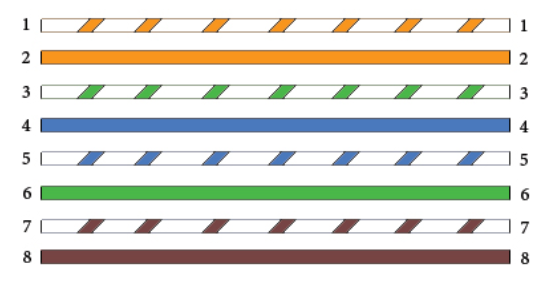
\includegraphics{Figures/straight.png}
    \caption{Straight-through cable connection in T-568B color-scheme}
    \label{fig:straight}
\end{figure}
\subsection*{Cross-over cable}
LAN cable where the transmitting and receiving terminals are interconnected rather than just straight forward connection is called cross-over cable. In this configuration, pin 1 on one end is connected to pin 3 on the other, pin 2 on one end is connected to pin 6 on the other. Likewise, the pin 4 is connected to pin 7 and pin 5 to pin 8 resulting in a cross-over of the wires. This type of cable is used when there's a need to connect two host devices to each other. Say a laptop and a computer need to be connected to one another but without using a hub or a third network device. In such case, a cross-over cable enables full duplex network between the two hosts directly.
\begin{figure}[H]
    \centering
    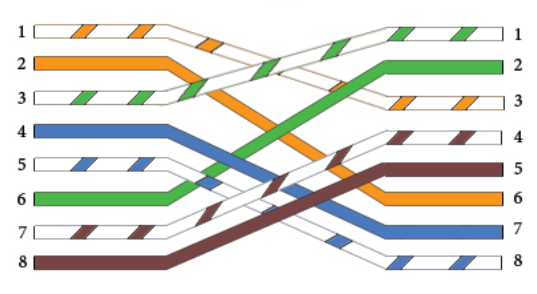
\includegraphics{Figures/cross.png}
    \caption{Cross-over cable connection in T-568B color-scheme}
    \label{fig:straight}\end{figure}
\section{Conclusion}
The lab experiment for Study of Network Architecture with Network Devices and Cables was concluded following the realization of the objectives. Various network devices such as hub, repeater, bridge, switch, router, and gateway were discussed. A more practical approach was chosen for the topics with images and discussions that matched real-life usage of those devices. LAN cable configurations were discussed along with the preparation guidelines. A faulty cable was then tested using the LAN cable tester following the aforementioned procedures. Once the problem was noted, the cable was fixed by replacing the RJ45 connector on one of its terminals using the crimping tool. Practical implementations of straight-through and cross-over cables were discussed and lab exercises that covered all the discussions were completed leading to the completion of the lab experiment.\end{document}